\subsection{Sub-Doppler cooling}
It is possible that the cooling below the doppler limit could be caused by a gradient force in the laser intensity.
Typically we expect to see our two laser fields with identical polarization, so they will form spatially standing waves.
If we make these polarizations orthogonal, there will be no spatial intensity modulation which surprisingly gives better results.
So this doesn't really seem to explain how we broke the doppler limit.

We next consider the additional energy levels of the atom, instead of looking at it as a two level system, we consider a hyperfinely split system (which has many energy levels).

We could also consider if there is a polarization gradient. If we have two conterporpogating fields with different polarizations then you find that the net polarization is circular:
\begin{align*}
	\bm{E}_l &= E_0\hat{e}_x e^{ikz} \\
	\bm{E}_r &= E_0\hat{e}_y e^{-ikz} \\
	\bm{E} &= \bm{E}_l + \bm{E}_r & \text{Assuming out of face for simplicity} \\
	\bm{E} &\propto (\hat{e}_x + i\hat{e}_y)\cos kz + i(\hat{e}_x - i\hat{e}_y)\sin kz \\
	\bm{E} &\propto \hat{e}_+\cos kz + i\hat{e}_y\sin kz
\end{align*}
Which are circularly polarized waves, with the portion of each polarization varying spatially. These two different polarizations cause our system to couple to multiple states.
The process of optical pumping then governs a dissipative process using these mechanisms.

To fully charactorize this process we would need to look at Clebsch-Gordon coefficients for different transitions, but instead here we approach this with a simplified model.
We consider in our model the $J=\frac{1}{2}\to J=\frac{1}{2}$ transition. 
\begin{figure*}[h!]
	\centering
	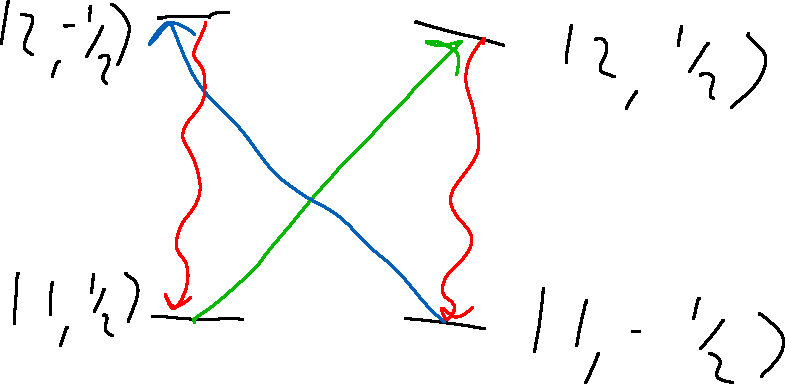
\includegraphics[width=10cm]{images/12-05-1.png}
	\caption*{Transitions for our model, in green is the $\sigma_+$ transition, in blue is the $\sigma_-$ transition and in red is the optical pumping transition}
\end{figure*}
As the atoms move around they reach the peak of their corresponding potentials due to the polarizations coopling to the other states.
At the peak they are most likely to be excited to a higher state, which then decays to a lower state that couples via the opposite polarization of light.
Therefore the atom finds itself at the bototom of a well, then they repeat this proces, losing $\frac{\hbar|\Omega_0|^2}{4|\delta|}$.
\begin{figure*}[h!]
	\centering
	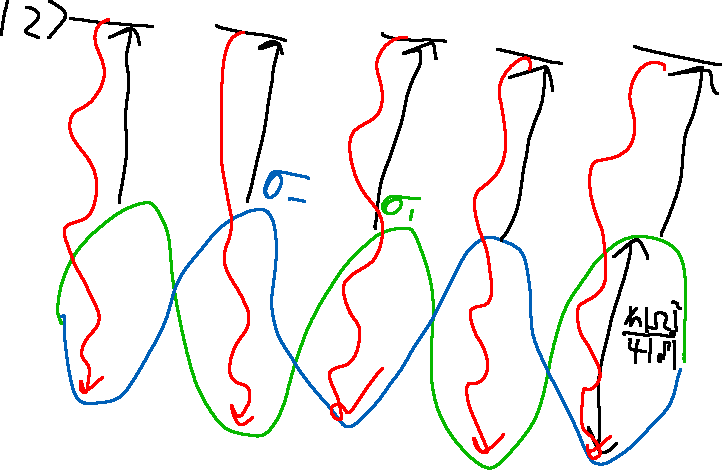
\includegraphics[width=10cm]{images/12-05-2.png}
	\caption*{Atoms in sysyphus cooling potential}
\end{figure*}
This process works well when $k_B T > \frac{\hbar |\Omega_0|^2}{4|\delta|}$. Additionally we have a recoil limit $\frac{(\hbar k)^2}{2M} = k_B T_r$.
This recoil limit is $T_R~1\mu K$.

Now we clearly want to concider how to circumvent this cooling limit. In order to do this we want to avoid spontaneous emission, and therefore avoid the excited state whenever possible.
In orer to avoid exciting the atom we utilize the dark state.

When we include the momentum in our state, we have the dark and bright states (when the fields are equal) are described by:
\begin{align*}
	\ket{D,p} &= \frac{1}{\sqrt{2}}(\ket{+1,p+\hbar k} - \ket{-1,p-\hbar k}) \\
	\ket{B,p} &= \frac{1}{\sqrt{2}}(\ket{+1,p+\hbar k} + \ket{-1,p-\hbar k})
\end{align*}
\begin{figure*}[h!]
	\centering
	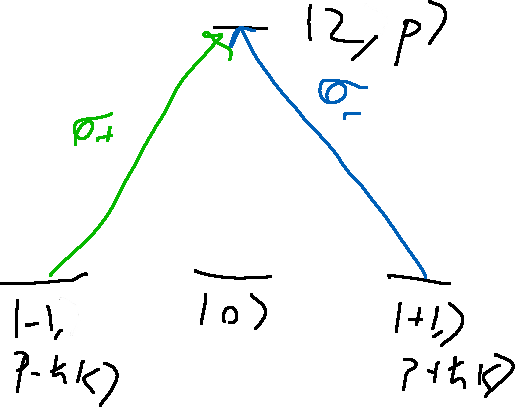
\includegraphics[width=10cm]{images/12-05-3.png}
	\caption*{Dark states in our sysyphus cooling setup}
\end{figure*}
We see that the $\ket{D,p}$ state is only dark if $p=0$. This allows for cooling because any state can be randomly put into $\ket{D,p}$ by random recoil, which will then stay in that state for all time since it is a dark state.
This is known as velocity selective CPT.

In trapped ions there is also the process of resolved sideband cooling.
